\title{CS4221/CS5421\\Database Applications Design and Tuning}

\subtitle{Tutorial 3: Dependency}

\author{Mark Meng Huasong}

\institute[National University of Singapore] % (optional, but mostly needed)
{
	School of Computing\\
	National University of Singapore
}

\titlegraphic{
	
\includegraphics[width=2cm]{nus-logo}
}

\date{Week 5, 2022 Spring}

\begin{frame}
	\titlepage
	\begin{tcolorbox}
		\begin{center}
			{\scriptsize \textcolor{red}{All the materials within presentation slides are protected by copyrights.\\
					It is forbidden by NUS to upload these materials to the Internet.}}
		\end{center}
	\end{tcolorbox}
\end{frame}


\section*{Question 1 Functional Dependencies}

\begin{frame}[fragile]{Question 1}
Consider the relational schema $R=\{A, B, C, D, E\}$ with the following set of functional dependencies.\\\vspace{5pt}
$\Sigma=\{\{A, B\} \rightarrow \{C\}, \{D\} \rightarrow \{D, B\}, \{B\} \rightarrow \{E\}, \{E\} \rightarrow \{D\}, \{A, B, D\} \rightarrow \{A, B, C, D\}\}$.
\end{frame}

\begin{frame}[fragile]{Question 1 (a-b) Attribute Closure \& Candidate Keys}
\textbf{(a) Compute all the closures of the the sets of attributes that are not equal to themselves, are not super-keys or are candidate keys.} \\
\textbf{What information is not essential and could be removed.}\vspace{15pt}

\textbf{Solution}: \vspace{3pt}

\begin{columns}[t]
	\column{0.45\textwidth}
	\textcolor{gray}{\scriptsize \textit{(Let's start with single attribute first)}}\\
	\textcolor{gray}{$\{A\}^{+}= \{A\}$ \scriptsize \textit{(omitted)}}\\	
	$\{B\}^{+}= \{B, D, E\}$\\	
	\textcolor{gray}{$\{C\}^{+}= \{C\}$ \scriptsize \textit{(omitted)}}\\
	$\{D\}^{+}= \{B, D, E\}$\\
	$\{E\}^{+}= \{B, D, E\}$\\ \vspace{5pt}
	\textcolor{gray}{\textit{\scriptsize (Two attributes' combination)}}\\
	$\underline{\{A, B\}^{+}}= \{A, B, C, D, E\}$\\
	\textcolor{gray}{$\{A, C\}^{+}= \{A, C\}$ \scriptsize \textit{(omitted)}}\\
	$\underline{\{A, D\}^{+}}= \{A, B, C, D, E\}$\\
	$\underline{\{A, E\}^{+}}= \{A, B, C, D, E\}$
	\column{0.45\textwidth}	
	$\{B, C\}^{+}= \{B, C, D, E\}$\\
	$\{B, D\}^{+}= \{B, D, E\}$\\
	$\{B, E\}^{+}= \{B, D, E\}$\\
	$\{C, D\}^{+}= \{B, C, D, E\}$\\
	$\{C, E\}^{+}= \{B, C, D, E\}$\\
	$\{D, E\}^{+}= \{B, D, E\}$\\
	 \vspace{5pt}
	Other attribute closures need not be computed.
\end{columns}
\end{frame}

\begin{frame}[fragile]{Question 1 (a) Cont.}
	We see the candidate keys are $\{A,B\}$, $\{A,D\}$ and $\{A,E\}$.\\
	\textcolor{blue}{This is the answer for 1(b)}\\
	\vspace{15pt}
	\textit{We can also visualize the FD as a figure below:}\\
	\begin{figure}
		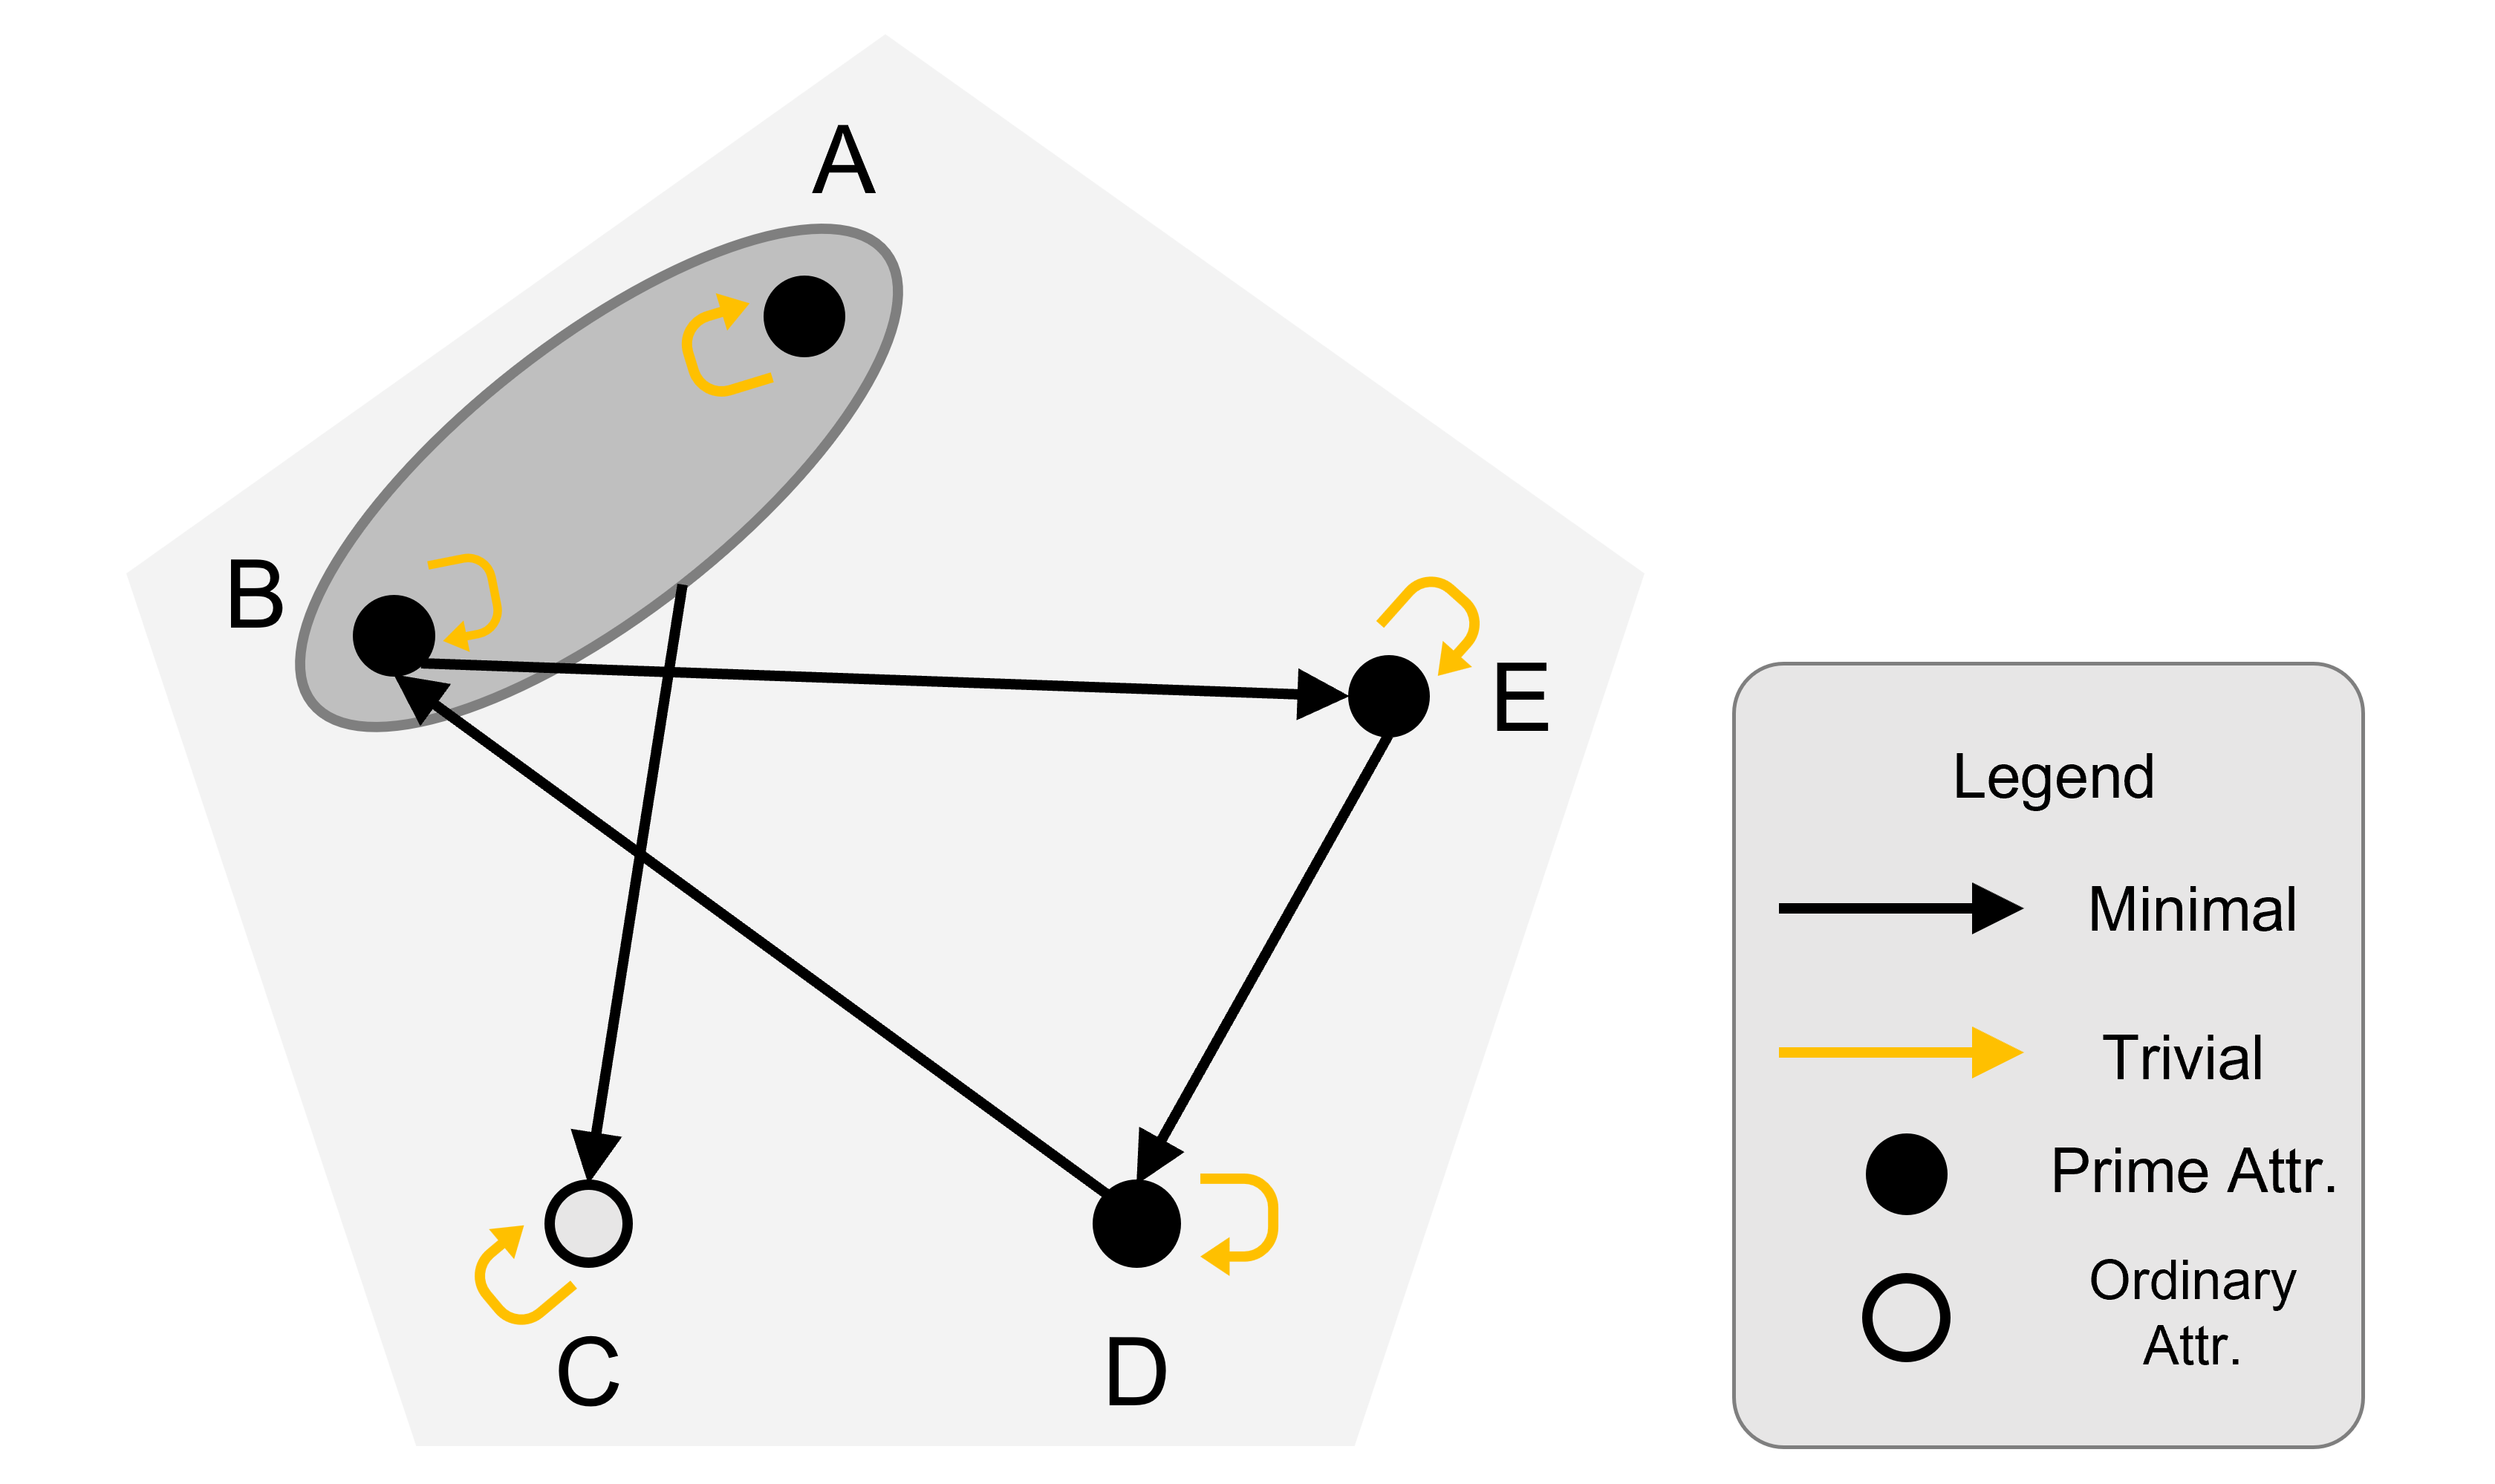
\includegraphics[width=0.85\textwidth, trim=0 0 0 0, clip]{4221-t3/images/q1.png}
	\end{figure}
\end{frame}

\begin{frame}[fragile]{Question 1 (a) Cont.}
	Now let's remove those information that is not essential from this closure:\\\vspace{3pt}
	We can remove from the RHS the members of the set on the LHS, as it also keeps all the essential information:\\\vspace{6pt}
	\begin{columns}[t]
		\column{0.45\textwidth}
		$\{A, B\}^{+}= \{C, D, E\}$\\
		$\{A, D\}^{+}= \{B, C, E\}$\\
		$\{A, E\}^{+}= \{B, C, D\}$\\
		$\{B\}^{+}= \{D, E\}$\\
		$\{D\}^{+}= \{B, E\}$\\
		$\{E\}^{+}= \{B, D\}$\\ 
		$\{B, C\}^{+}= \{D, E\}$\\
		$\{B, D\}^{+}= \{E\}$\\
		\column{0.45\textwidth}	
		$\{B, E\}^{+}= \{D\}$\\
		$\{C, D\}^{+}= \{B, E\}$\\
		$\{C, E\}^{+}= \{B, D\}$\\
		$\{D, E\}^{+}= \{B\}$\\
		$\{B, C, D\}^{+}= \{E\}$\\
		$\{B, C, E\}^{+}= \{D\}$\\
		$\{C, D, E\}^{+}= \{B\}$		
	\end{columns}
\end{frame}

\begin{frame}[fragile]{Question 1 (a) Cont.}
	Remark: We can even remove an equality if the LHS is a superset of another equality LHS and its RHS is a subset of the RHS (e.g., give $\{E\}^{+}= \{B, D\}$ and $\{C, D, E\}^{+}= \{B\}$, we can omit the second one). It also keeps all the essential information:\\\vspace{6pt}

	$\{A, B\}^{+}= \{C, D, E\}$\\
		$\{A, D\}^{+}= \{B, C, E\}$\\
		$\{A, E\}^{+}= \{B, C, D\}$\\
		$\{B\}^{+}= \{D, E\}$\\
		$\{D\}^{+}= \{B, E\}$\\
		$\{E\}^{+}= \{B, D\}$\\ \vspace{7pt}
	
	\textbf{(b) What are the candidate keys of $R$ with $\Sigma$?}\\\vspace{3pt}
	The candidate keys are $\{A,B\}$, $\{A,D\}$ and $\{A,E\}$.\\
\end{frame}

\begin{frame}[fragile]{Question 1 (c-d) Minimal Cover}
	(c) Find a minimal cover of $R$ with $\Sigma$ that can be reached from $\Sigma$ using the algorithm from the lecture.\\ \vspace{5pt}
	\textbf{Solution}: The candidate keys are $\{A, E\}$ and $\{B, E\}$. \\\vspace{35pt}

	(d) Find all the minimal covers of $R$ with $\Sigma$\\ \vspace{5pt}
	\textbf{Solution}: The prime attributes are $A$, $B$ and $E$.
\end{frame}

\begin{frame}[fragile]{Question 1 (e) Armstrong Axioms}
	(e) Prove, using the three Armstrong axioms, that the following set of functional dependencies is equivalent to $\Sigma$. \\\vspace{5pt}
	$\Sigma''''=\{\{A, B\} \rightarrow \{C, D, E\}, \{A, D\} \rightarrow \{B, C, E\}, \{A, E\} \rightarrow \{B, C, D\}, \{B\} \rightarrow \{D, E\}, \{D\} \rightarrow \{B, E\}, \{E\} \rightarrow \{B, D\}\}$.\\\vspace{5pt}
	 \vspace{5pt}
	\textbf{Solution}: The candidate keys are $\{A, E\}$ and $\{B, E\}$. \\\vspace{35pt}
	
\end{frame}

\section*{Question 2 Minimal Cover}

\begin{frame}[fragile]{Question 2 (a) Minimal Cover.}
	(a) Compute a minimal cover of $R$ with $\Sigma$.\vspace{10pt}

	\textbf{Solution}: \\\vspace{3pt}
	We start from $\Sigma$: \\\vspace{5pt}
	$\{A\} \rightarrow \{A, B, C\}$\\
	$\{A, B\} \rightarrow \{A\}$\\
	$\{B, C\} \rightarrow \{A, D\}$\\
	$\{B\} \rightarrow \{A, B\}$\\
	$\{C\} \rightarrow \{D\}$\\\vspace{5pt}
	Step 1, we simplify the right-hand sides:\\\vspace{3pt}
	\begin{columns}[t]
	\column{0.45\textwidth}
	$\{A\} \rightarrow \{A\}$\\
	$\{A\} \rightarrow \{B\}$\\
	$\{A\} \rightarrow \{C\}$\\
	$\{A, B\} \rightarrow \{A\}$\\
	$\{B, C\} \rightarrow \{A\}$
	\column{0.45\textwidth}
	$\{B, C\} \rightarrow \{D\}$\\
	$\{B\} \rightarrow \{A\}$\\
	$\{B\} \rightarrow \{B\}$\\
	$\{C\} \rightarrow \{D\}$
	\end{columns}
\end{frame}

\begin{frame}[fragile]{Question 2 (a) Cont.}
	Step 2, we simplify the left-hand sides:\\\vspace{3pt}
	$\{A\} \rightarrow \{A\}$.\\	
	$\{A\} \rightarrow \{B\}$.\\	
	$\{A\} \rightarrow \{C\}$.\\	
	$\{A,\cancel{B}\} \rightarrow \{A\}$ because $\{A\} \rightarrow \{A\}$.\\	
	$\{B, \cancel{C}\} \rightarrow \{A\}$ because $\{B\} \rightarrow \{A\}$.\\	
	$\{B, \cancel{C}\} \rightarrow \{D\}$ because $\{B\} \rightarrow \{D\}$ \\\vspace{3pt}
	(we could also do $\{\cancel{B}, C\} \rightarrow \{D\}$ because $\{C\} \rightarrow \{D\}$). Note that we know that $\{B\} \rightarrow \{D\}$ because $\{B\}^{+}= \{A, B, C, D\}$.\\\vspace{3pt}
	$\{B\} \rightarrow \{A\}$.\\
	$\{B\} \rightarrow \{B\}$.\\
	$\{C\} \rightarrow \{D\}$.
\end{frame}

\begin{frame}[fragile]{Question 2 (a) Cont.}
	Step 3, we simplify the set:\\\vspace{3pt}
	$\cancel{\{A\} \rightarrow \{A\}}$ because it is trivial.\\	
	$\{A\} \rightarrow \{B\}$.\\	
	$\{A\} \rightarrow \{C\}$.\\	
	$\{B\} \rightarrow \{A\}$.\\	
	$\cancel{\{B\} \rightarrow \{D\}}$ because it can be derived from the others.\\	
	$\cancel{\{B\} \rightarrow \{B\}}$ $\cancel{\{A\} \rightarrow \{A\}}$.\\	
	$\{C\} \rightarrow \{D\}$.\\\vspace{5pt}
	
	\textbf{The result is:} \\\vspace{3pt}
	$\{A\} \rightarrow \{B\}$\\	
	$\{A\} \rightarrow \{C\}$\\	
	$\{B\} \rightarrow \{A\}$\\
	$\{C\} \rightarrow \{D\}$
\end{frame}

\begin{frame}[fragile]{Question 2 (a) Cont.}
	\begin{alertblock}{Notice}
	Note that there can be other minimal covers that the algorithm can compute by considering the functional dependencies in a different order at each step of the algorithm. This is not the case in the example.
	\end{alertblock}\vspace{5pt}

	However, there is a minimal cover that the algorithm cannot compute:\\\vspace{5pt}
	$\{A\} \rightarrow \{B\}$\\
	$\{B\} \rightarrow \{A\}$\\
	$\{B\} \rightarrow \{C\}$\\
	$\{C\} \rightarrow \{D\}$\\\vspace{10pt}	
	If the algorithm starts from $\Sigma^{+}$, then it can find all minimal covers.
\end{frame}

\begin{frame}[fragile]{Question 2 (b)}
	(b) Compute a compact minimal cover of $R$ with $\Sigma$.\vspace{10pt}
	
	\textbf{Solution}: \\\vspace{5pt}
	Given the minimal cover of $R$ with $\Sigma$:\\\vspace{3pt}
	$\{A\} \rightarrow \{B\}$\\	
	$\{A\} \rightarrow \{C\}$\\	
	$\{B\} \rightarrow \{A\}$\\
	$\{C\} \rightarrow \{D\}$\\\vspace{5pt}
	The \textbf{compact minimal cover} is:\\\vspace{3pt}
	$\{A\} \rightarrow \{B, C\}$\\	
	$\{B\} \rightarrow \{A\}$\\	
	$\{C\} \rightarrow \{D\}$
\end{frame}


\begin{frame}{}
	\centering  
	For any further question, please feel free to email me:\vspace{10pt}
	
	huasong.meng@u.nus.edu\\\vspace{3pt}
	% Or you can whatsapp/wechat me via: 81028639 \vspace{20pt}
	
	\begin{tcolorbox}
		\begin{center}
			\textcolor{red}{Copyright 2021 Mark H. Meng. All rights reserved.}
		\end{center}
	\end{tcolorbox}
\end{frame}